%%%
% Plantilla de Presentación
% Modificación de una plantilla de Latex de LaTeXTemplates para adaptarla 
% al castellano y a las necesidades de escribir informática y matemáticas.
%
% Editada por: Mario Román
%
% License:
% CC BY-NC-SA 3.0 (http://creativecommons.org/licenses/by-nc-sa/3.0/)
%%%

%%%%%%%%%%%%%%%%%%%%%%%%%%%%%%%%%%%%%%%%%
% Beamer Presentation
% LaTeX Template
% Version 1.0 (10/11/12)
%
% This template has been downloaded from:
% http://www.LaTeXTemplates.com
%
% License:
% CC BY-NC-SA 3.0 (http://creativecommons.org/licenses/by-nc-sa/3.0/)
%
%%%%%%%%%%%%%%%%%%%%%%%%%%%%%%%%%%%%%%%%%

%----------------------------------------------------------------------------------------
%	PAQUETES Y CONFIGURACIÓN DEL DOCUMENTO
%----------------------------------------------------------------------------------------

\documentclass{beamer}

%% Configuración de la presentación
\mode<presentation> {
  %%% Selección de estilo
  % The Beamer class comes with a number of default slide themes
  % which change the colors and layouts of slides. Below this is a list
  % of all the themes, uncomment each in turn to see what they look like.

  %\usetheme{default}
  %\usetheme{AnnArbor}
  %\usetheme{Antibes}
  %\usetheme{Bergen}
  %\usetheme{Berkeley}
  %\usetheme{Berlin}
  %\usetheme{Boadilla}
  %\usetheme{CambridgeUS}
  %\usetheme{Copenhagen}
  %\usetheme{Darmstadt}
  %\usetheme{Dresden}
  %\usetheme{Frankfurt}
  %\usetheme{Goettingen}
  %\usetheme{Hannover}
  %\usetheme{Ilmenau}
  %\usetheme{JuanLesPins}
  %\usetheme{Luebeck}
  \usetheme{Madrid}
  %\usetheme{Malmoe}
  %\usetheme{Marburg}
  %\usetheme{Montpellier}
  %\usetheme{PaloAlto}
  %\usetheme{Pittsburgh}
  %\usetheme{Rochester}
  %\usetheme{Singapore}
  %\usetheme{Szeged}
  %\usetheme{Warsaw}

  %% Selección de color
  % As well as themes, the Beamer class has a number of color themes
  % for any slide theme. Uncomment each of these in turn to see how it
  % changes the colors of your current slide theme.

  %\usecolortheme{albatross}
  %\usecolortheme{beaver}
  %\usecolortheme{beetle}
  %\usecolortheme{crane}
  %\usecolortheme{dolphin}
  %\usecolortheme{dove}
  %\usecolortheme{fly}
  %\usecolortheme{lily}
  %\usecolortheme{orchid}
  %\usecolortheme{rose}
  %\usecolortheme{seagull}
  %\usecolortheme{seahorse}
  %\usecolortheme{whale}
  %\usecolortheme{wolverine}

  %% Configuración del pie de línea
  %\setbeamertemplate{footline} % To remove the footer line in all slides uncomment this line
  %\setbeamertemplate{footline}[page number] % To replace the footer line in all slides with a simple slide count uncomment this line
  %\setbeamertemplate{navigation symbols}{} % To remove the navigation symbols from the bottom of all slides uncomment this line
}

%% Fuentes de tamaño arbitrario
\usepackage{lmodern}

%% Gráficos
\usepackage{graphicx} % Allows including images
\usepackage{booktabs} % Allows the use of \toprule, \midrule and \bottomrule in tables

%%% Castellano.
% noquoting: Permite uso de comillas no españolas.
% lcroman: Permite la enumeración con numerales romanos en minúscula.
% fontenc: Usa la fuente completa para que pueda copiarse correctamente del pdf.
\usepackage[spanish,es-noquoting,es-lcroman]{babel}
\usepackage[utf8]{inputenc}
\usepackage[T1]{fontenc}
\selectlanguage{spanish}
\unaccentedoperators

% Algoritmos
\usepackage{algorithm}
\usepackage{algpseudocode}

%----------------------------------------------------------------------------------------
%	TÍTULO
%----------------------------------------------------------------------------------------

\title[Primalidad en Tiempo Polinomial]{Primalidad en Tiempo Polinomial} % The short title appears at the bottom of every slide, the full title is only on the title page

\author{Francisco Gallego Salido} % Your name
\institute[UGR] % Your institution as it will appear on the bottom of every slide, may be shorthand to save space
{
  Universidad de Granada \\ % Your institution for the title page
  \medskip
  \textit{fgallego@correo.ugr.es} % Your email address
}
\date{\today} % Date, can be changed to a custom date



\begin{document}

%% Diapositiva de título.
\begin{frame}
\titlepage % Print the title page as the first slide
\end{frame}

%% Diapositiva de contenidos.
% Throughout your presentation, if you choose to use \section{} and \subsection{} commands, 
% these will automatically be printed on this slide as an overview of your presentation
\begin{frame}
  \frametitle{Contenidos} % Table of contents slide, comment this block out to remove it
  \tableofcontents
\end{frame}



%----------------------------------------------------------------------------------------
%	PRESENTACIÓN
%----------------------------------------------------------------------------------------

\section{Tests de Primalidad}

\begin{frame}
	\centering
	\begin{Huge}
		Tests de Primalidad
	\end{Huge}
\end{frame}

\subsection{Introducción}

\begin{frame}
	\centering
	\begin{Large}
		Introducción
	\end{Large}
\end{frame}

\begin{frame}{¿Qué son los números primos?}
	Un número primo es aquel que solo es divisible por $1$ o por sí mismo.\break
	
	\begin{example}
		El número 5 es primo porque solo es divisible por $1$ y $5$.
	\end{example}
	
	\begin{example}
		El número $12$ no es primo porque es divisible por $2$, $3$, $4$ y $6$, que son distintos de $1$ y $12$.
	\end{example}
\end{frame}

\begin{frame}{¿Qué es un test de primalidad?}
	Un test de primalidad es un algoritmo que nos permite determinar si un número es primo o no.\break
	
	El test más básico es el que se deriva de la definición de primalidad, cuya complejidad es $O(\sqrt{(n)})$:
	
	\begin{itemize}[<+(1)->]
		\item Comprobar todos los números menores que $\lfloor\sqrt{n}\rfloor$ y ver si alguno divide a $n$.
		
		\item Si ninguno lo divide, $n$ es primo.
		
		\item Si alguno lo divide, $n$ es compuesto.
	\end{itemize}
\end{frame}

\subsection{Pequeño Teorema de Fermat}

\begin{frame}
	\centering
	\begin{Large}
		Pequeño Teorema de Fermat
	\end{Large}
\end{frame}

\begin{frame}{Pequeño Teorema de Fermat}
	\onslide<1->Un test mucho más eficiente es el que se deriva del \textit{Pequeño Teorema de Fermat}.\break
	
	\onslide<2->
	\begin{theorem}[Pequeño Teorema de Fermat]
		Si $n$ es primo, entonces $a^n \equiv a \mod(n)$ para todo $a \in \mathbb{Z}$.
	\end{theorem}
	
	\onslide<3->El test consiste en comprobar varios valores de $a$ y vemos si se cumple la congruencia.\break
	
	\onslide<4->Si falla para algún $a$, entonces $n$ es compuesto. En caso contrario, $n$ probablemente sea primo.
\end{frame}

\begin{frame}{Problema}
	\onslide<1->No es cierto en general que si $a^n \equiv a \mod(n)$ para todo $a \in \mathbb{Z}$, entonces $n$ sea primo.\break
	
	\onslide<2->De hecho, existe un conjunto de números que no son primos para los que el \textit{Pequeño Teorema de Fermat} siempre se cumple.\break
	
	\onslide<3->A dicho conjunto se le conoce como \textit{Números de Charmichael}, donde $561 = 3\cdot11\cdot17$ es el primer elemento de dicho conjunto.
\end{frame}

\section{Algoritmo AKS}

\begin{frame}
	\centering
	\begin{Huge}
		Algoritmo AKS
	\end{Huge}
\end{frame}

\begin{frame}{Historia}
	\onslide<1->El algoritmo \textbf{AKS} debe su nombre a los tres matemáticos que lo descubrieron: Manindra Agrawal, Neeraj Kayal y Nitin Saxena.\break
	
	\onslide<2->Se trata del primer test de primalidad que cumple todas las propiedades deseadas:\break
	
	\begin{itemize}[<+(2)->]
		\item \textbf{General}. Es válido para cualquier entrada.
		
		\item \textbf{Determinista}. Determina con una probabilidad del $100\%$ la primalidad de un número.
		
		\item \textbf{Polinómico}. La complejidad asintótica del test es polinómica en el número de cifras.
		
		\item \textbf{Incondicional}. La validez del test no depende de resultados no probados.
	\end{itemize}
\end{frame}

\subsection{Introducción}

\begin{frame}
	\centering
	\begin{Large}
		Introducción
	\end{Large}
\end{frame}

\begin{frame}{Idea Principal}
	\onslide<1->El \textit{Pequeño Teorema de Fermat} no proporciona un test válido, pero una versión general suya sí. Sea el siguiente teorema:\break
	
	\onslide<2->
	\begin{theorem}
		Sea $n > 1$ y $a \in \mathbb{Z}$. Entonces $n$ es primo si, y solo si, se cumple
		
		\begin{equation*}
		(X + a)^n \equiv X^n + a \mod(n)
		\end{equation*}
	\end{theorem}
	
	\onslide<3->Un test que se deriva de esta propiedad es simplemente comprobar si la congruencia se cumple para algún $a$.\break
	
	\onslide<4->Si se cumple, entonces $n$ es primo. En caso contrario, $n$ es compuesto.
\end{frame}

\begin{frame}{¿Es este test polinómico?}
	Un problema que tiene este test es que tiene complejidad $\Omega(n)$, pues hay que evaluar $n$ coeficientes de los polinomios resultantes.\break
	
	Este test es muy ineficiente y lejos de ser polinómico en la cantidad de cifras.\break
	
	\onslide<2->¿Podemos reducir el número de coeficientes a evaluar?
\end{frame}

\begin{frame}{Solución}
	\onslide<1->Si la congruencia anterior la evaluamos módulo $(X^r - 1, n)$ para algún $r$ escogido apropiadamente, podremos reducir el número de coeficientes. Sea pues la siguiente congruencia:\break
	
	\onslide<2->
	\begin{equation*}
	(X + a)^n \equiv X^n + a \mod(X^r - 1, n)
	\end{equation*}
	
	\onslide<3->El problema de esta congruencia es que, aunque se sigue cumpliendo cuando $n$ es primo, algunos compuestos la cumplen también para algunos valores de $a$ y $r$.\break
	
	\onslide<4->Escogiendo apropiadamente $r$ y probando para ciertos valores de $a$, si se cumple entonces la congruencia anterior, podemos asegurar que $n$ es una potencia de un primo.\break
	
	\onslide<5->Dichos $r$ y $a$ se pueden elegir de forma que la complejidad del test sea polinómica.
\end{frame}

\subsection{El Algoritmo}

\begin{frame}
	\centering
	\begin{Large}
		El Algoritmo
	\end{Large}
\end{frame}

\begin{frame}[fragile]{Pasos del Algoritmo AKS}
	\begin{algorithm}[H]
		\caption{AKS}
		\begin{algorithmic}
			\Procedure{IsPrime}{$n$}\Comment{Comprobar si $n > 1$ es un número primo}
				\State \textbf{if} $n = a^b$ con $a, b > 1$ \Return{COMPUESTO}\Comment{Paso 1}\medskip
				\State Encontrar el menor $r$ tal que $ord_r(n) > \log^2(n)$.\Comment{Paso 2}\medskip
				\State \textbf{if} $1 < (a, n) < n$ para algún $a \leq r$ \Return{COMPUESTO}\Comment{Paso 3}\medskip
				\State \textbf{if} $n \leq r$ \Return{PRIMO}\Comment{Paso 4}\medskip
				\For{$a = 1$ hasta $\lfloor \sqrt{\phi(r)}\log(n) \rfloor$}\Comment{Paso 5}
					\State \textbf{if} $(X + a)^n \not\equiv X^n + a \mod(n, X^r - 1)$ \Return{COMPUESTO}
				\EndFor\medskip
				\State \Return{PRIMO}\Comment{Paso 6}
			\EndProcedure
		\end{algorithmic}
	\end{algorithm}
\end{frame}

\begin{frame}{Ejemplo}
	Sea el número $31$, el cual ya sabemos que es primo.
	
	\begin{enumerate}[<+(1)->]
		\item $31$ no es una potencia perfecta. Pasamos al siguiente paso.
		
		\item El menor $r$ es $29$, pues $ord_{29}(31) = 28 > \log^2(31) \simeq 24.54$.
		
		\item $(a, 31) = 1$ para todo $a \leq 29$. Pasamos al siguiente paso.
		
		\item $31 \not\leq 29$. Pasamos al siguiente paso.
		
		\item
		
		\begin{itemize}
			\item $\lfloor\sqrt{\phi(r)}\log(n)\rfloor = 26$.
			
			\item $(X + a)^{31} = x^2 + a^{31}$ módulo $(X^{29}-1, 31)$.
			
			\item $X^{31} + a = x^2 + a$ módulo $(X^{29}-1, 31)$.
			
			\item $a^{31} \equiv a \mod(X^{29}-1, 31)$ para todo $1 \leq a \leq 26$. Pasamos al siguiente paso
		\end{itemize}
		
		\item Hemos llegado al último paso, por lo que $31$ es primo.
	\end{enumerate}
\end{frame}

\subsection{Complejidad}

\begin{frame}
	\centering
	\begin{Large}
		Complejidad
	\end{Large}
\end{frame}

\begin{frame}{Complejidad Paso a Paso}
	Cada paso tiene un complejidad determinada:\break
	
	\begin{itemize}[<+(1)->]
		\item $O^\sim(\log^3(n))$.
		\item $O^\sim(\log^7(n))$.
		\item $O^\sim(\log^6(n))$.
		\item $O(\log(n))$.
		\item $O^\sim(\log^{21/2}(n))$.
		\item $O(1)$.
	\end{itemize}
\end{frame}

\begin{frame}{Complejidad Total}
	\onslide<1->La complejidad del quinto paso es la más alta, luego el algoritmo \textbf{AKS} tiene una complejidad algorítmica de $O^\sim(\log^{21/2}(n))$.\break
	
	\onslide<2->Usando \textit{Teoría de Cribas} se puede probar que $r = O(\log^3(n))$, reduciendo la complejidad hasta $O^\sim(\log^{15/2}(n))$.\break
	
	\onslide<3->Bajo ciertas hipótesis no probadas (como puede ser la \textit{Hipótesis Generalizada de Riemann}), se puede probar que $r = O(\log^2(n))$, reduciendo una vez más la complejidad hasta $O^\sim(\log^6(n))$.
\end{frame}

\section{Comparaciones}

\begin{frame}
	\centering
	\begin{Huge}
		Comparaciones
	\end{Huge}
\end{frame}

\begin{frame}{Candidatos}
	\onslide<1->Vamos a comparar el algoritmo AKS con dos tests probabilísticos:\break
	
	\begin{itemize}[<+(1)->]
		\item Test de \textit{Miller-Rabin} con $40$ rondas.
		
		\item Test de \textit{Solovay-Strassen} con $80$ rondas.
	\end{itemize}
\end{frame}

\subsection{Primos}

\begin{frame}
	\centering
	\begin{Large}
		Primos
	\end{Large}
\end{frame}

\begin{frame}{Conjunto de Prueba}
	Los números primos con los que se hacen las pruebas tienen una cantidad incremental de bits.\break
	
	Por ejemplo, el $7$ es el mayor primo con $3$ bits, $31$ el mayor primo con $5$ bits, $2147483647$ el mayor primo con $32$ bits, etc.\break
\end{frame}

\begin{frame}{Comparación Números Primos}
	\begin{alertblock}{}
		\begin{center}
			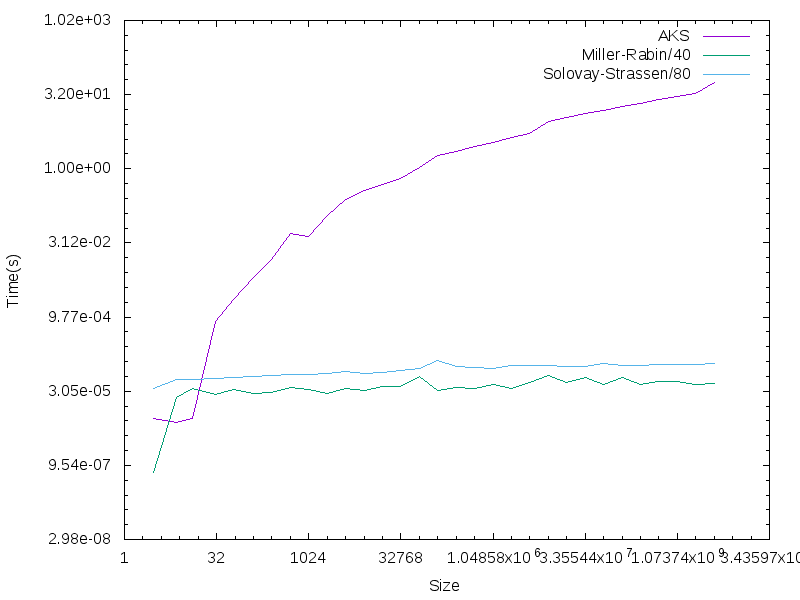
\includegraphics[scale=0.40]{../Memoria/img/graphs/aks-probs-primes-mean}
		\end{center}
	\end{alertblock}
\end{frame}

\subsection{Potencias Perfectas}

\begin{frame}
	\centering
	\begin{Large}
		Potencias Perfectas
	\end{Large}
\end{frame}

\begin{frame}{Conjunto de Prueba}
	Las potencias perfectas que usaremos serán con los primos presentados anteriorimente, y consisten de dos conjuntos:\break
	
	\begin{itemize}[<+(1)->]
		\item Primos de hasta $16$ bits elevados a $100$.
		
		\item Primos de entre $192$ y $256$ bits elevados a $5$.
	\end{itemize}
\end{frame}

\begin{frame}{Comparación Potencias Perfectas 1}
	\begin{alertblock}{}
		\begin{center}
			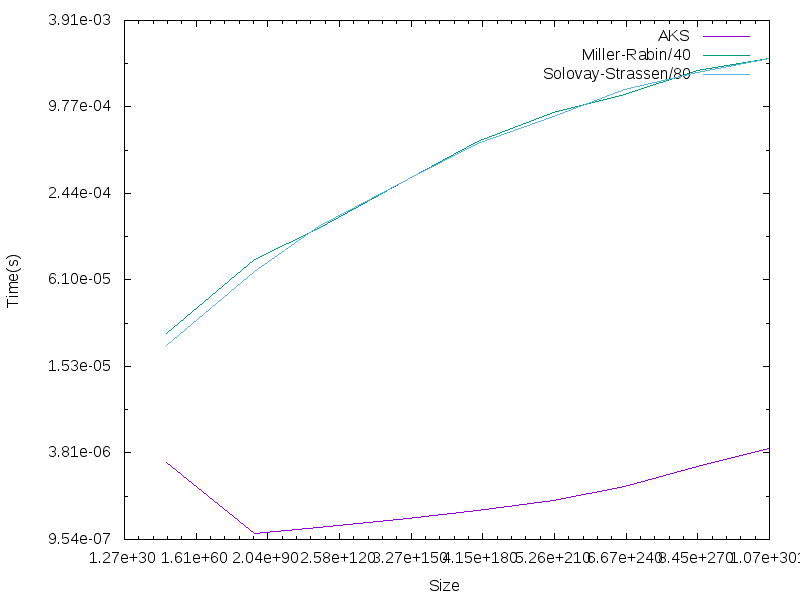
\includegraphics[scale=0.40]{../Memoria/img/graphs/aks-probs-powers-100-mean}
		\end{center}
	\end{alertblock}
\end{frame}

\begin{frame}{Comparación Potencias Perfectas 2}
	\begin{alertblock}{}
		\begin{center}
			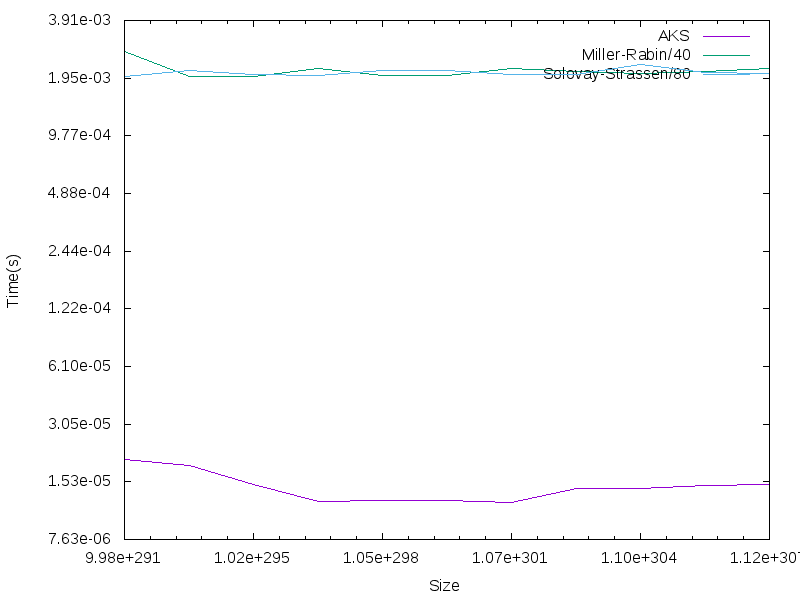
\includegraphics[scale=0.40]{../Memoria/img/graphs/aks-probs-powers-5-mean}
		\end{center}
	\end{alertblock}
\end{frame}

\subsection{Compuestos No Potencias Perfectas}

\begin{frame}
	\centering
	\begin{Large}
		Compuestos No Potencias Perfectas
	\end{Large}
\end{frame}

\begin{frame}{Conjunto de Prueba}
	Los números compuestos que usaremos en estas comparaciones serán producto de los primos mencionados anteriormente. Hay dos conjuntos:\break
	
	\begin{itemize}[<+(1)->]
		\item Primos de entre $32$ y $42$ bits multiplicados por un primo de $16$ bits.
		
		\item Primos de entre $32$ y $42$ bits multiplicados por un primo de $32$ bits.
	\end{itemize}
\end{frame}

\begin{frame}{Comparación Compuestos No Potencias Perfectas 1}
	\begin{alertblock}{}
		\begin{center}
			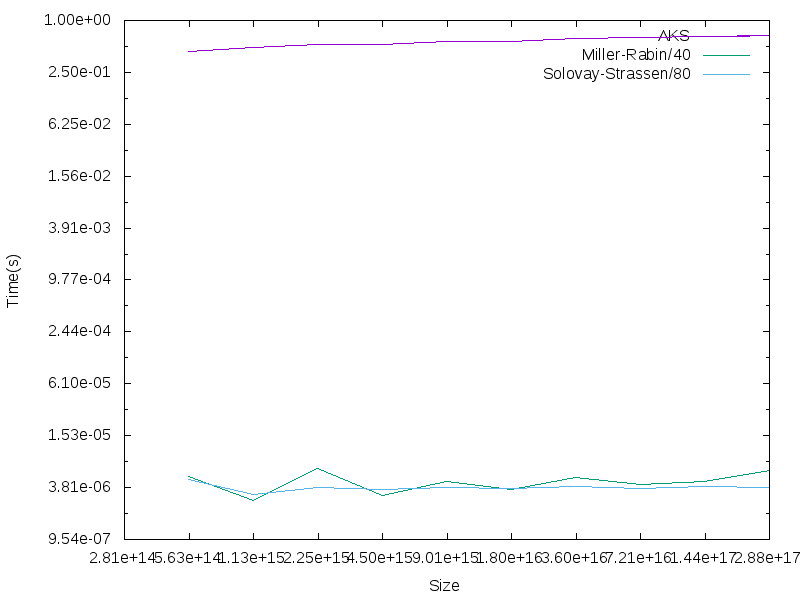
\includegraphics[scale=0.40]{../Memoria/img/graphs/aks-probs-comps-16-mean}
		\end{center}
	\end{alertblock}
\end{frame}

\begin{frame}{Comparación Compuestos No Potencias Perfectas 1}
	\begin{alertblock}{}
		\begin{center}
			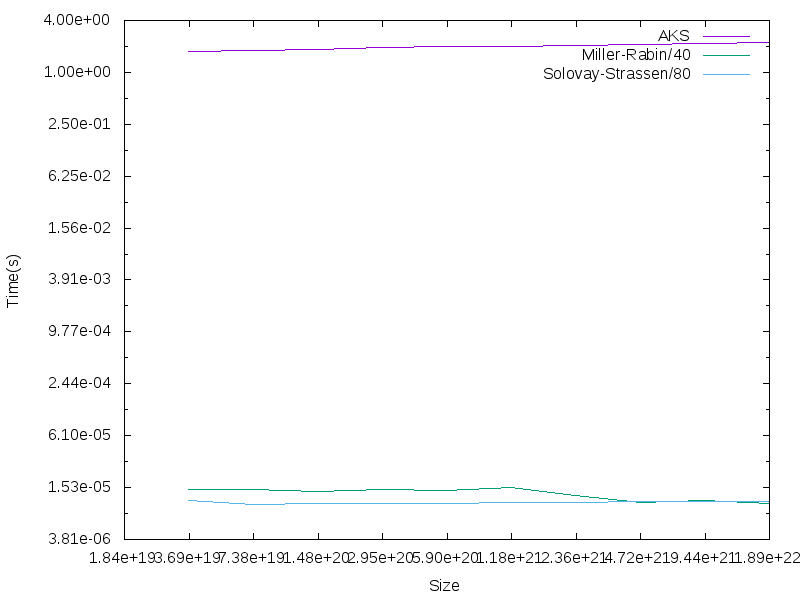
\includegraphics[scale=0.40]{../Memoria/img/graphs/aks-probs-comps-32-mean}
		\end{center}
	\end{alertblock}
\end{frame}

\section{Conclusiones}

\begin{frame}
	\centering
	\begin{Huge}
		Conclusiones
	\end{Huge}
\end{frame}

\begin{frame}{Conclusiones}
	\onslide<1->El test es brillante desde el punto de vista matemático, ya que la prueba de la validez del test usa herramientas elementales.\break
	
	\onslide<2->Sin embargo, a pesar de ser un test polinómico, en la práctica queda muy por detrás de otros test usados en la actualidad.
\end{frame}

%------------------------------------------------

%% Bibliografía
\begin{frame}
\frametitle{Referencias}
\footnotesize{
	\begin{thebibliography}{99} % Beamer does not support BibTeX so references must be inserted manually as below
		\bibitem[AKS04a]{AKS2004}
		Manindra Agrawal, Neeraj Kayal, and Nitin Saxena.
			\newblock {PRIMES} is in {P}.
			\newblock {\em Ann. of Math. (2)}, 160(2):781--793, 2004.
		\bibitem[AKS19]{AKS2019}
		Manindra Agrawal, Neeraj Kayal, and Nitin Saxena.
			\newblock Errata: {PRIMES} is in {P}.
			\newblock {\em Ann. of Math. (2)}, 189(1):317--318, 2019.
		\bibitem[Sal]{fgallego_tfg_github}
		Francisco~Gallego Salido.
			\newblock Tfg.
			\newblock \url{https://github.com/fgallegosalido/TFG}.
	\end{thebibliography}
}
\end{frame}

%------------------------------------------------

\begin{frame}
\Huge{\centerline{Fin}}
\end{frame}

%----------------------------------------------------------------------------------------

\end{document} 